\documentclass{beamer}

\usepackage[utf8]{inputenc}
\usetheme{metropolis}     
\usepackage{minted}
\usepackage{verbatim}
%\beamertemplatenavigationsymbolsempty
%\setbeamertemplate{footline}[frame number]


%Information to be included in the title page:
\title{Introduction to writing in LaTeX}
\author{Akos Mate}
\institute{Central European University}
\date{2019 January}


\begin{document}

\frame{\titlepage}

\section{Introduction}

%%%%%%%%%%%%%%%%%%%%%%%%%%%%%%%%%%%%%%%%%%%%%%%%%%%%%%%%%%%%%%%%%%%%%%%%%%%%%%%%%
%%%%%%%%%%%%%%%%%%%%%%%%%%%%%%%%%%%%%%%%%%%%%%%%%%%%%%%%%%%%%%%%%%%%%%%%%%%%%%%%%

\begin{frame}
	\frametitle{Overview}
	\begin{enumerate}
		\item What is (La)Tex and why use it?
		\item Goal of the workshop
		\item Very short first steps to get set up
		\item Using citation manager and LaTeX together
		\item CEU LaTeX template
		\item some other things that might be useful
	\end{enumerate}
\end{frame}


%%%%%%%%%%%%%%%%%%%%%%%%%%%%%%%%%%%%%%%%%%%%%%%%%%%%%%%%%%%%%%%%%%%%%%%%%%%%%%%%%
%%%%%%%%%%%%%%%%%%%%%%%%%%%%%%%%%%%%%%%%%%%%%%%%%%%%%%%%%%%%%%%%%%%%%%%%%%%%%%%%%

\begin{frame}
\frametitle{What is LaTeX?}
	TeX is a typesetting system. LaTeX is a set of macros that allows you to deal with text only and leave the formatting headache behind. \pause
	\bigskip

	\textbf{Goal of the workshop:} \pause
	\begin{enumerate}
	\item to give enough intro that you can start writing your papers in LaTeX
	\end{enumerate}
\end{frame}

%%%%%%%%%%%%%%%%%%%%%%%%%%%%%%%%%%%%%%%%%%%%%%%%%%%%%%%%%%%%%%%%%%%%%%%%%%%%%%%%%
%%%%%%%%%%%%%%%%%%%%%%%%%%%%%%%%%%%%%%%%%%%%%%%%%%%%%%%%%%%%%%%%%%%%%%%%%%%%%%%%%

\begin{frame}
	\frametitle{Why use LaTeX?}
	Pros:
	\begin{itemize}
		\item Output looks professional \pause
		\item Platform independent and reproducible output \pause
		\item Document formatting is not an issue \pause
		\item Writing and text dominates the workflow \pause
	\end{itemize}
	\medskip

	Cons:
	\begin{itemize}
		\item Steep learning curve \pause
		\item Initially you get work done slower \pause
		\item Can be hard to step out of the WYSIWYG comfort zone \pause
		\item Formatting tables is truly painful
	\end{itemize}
\end{frame}


%%%%%%%%%%%%%%%%%%%%%%%%%%%%%%%%%%%%%%%%%%%%%%%%%%%%%%%%%%%%%%%%%%%%%%%%%%%%%%%%%
%%%%%%%%%%%%%%%%%%%%%%%%%%%%%%%%%%%%%%%%%%%%%%%%%%%%%%%%%%%%%%%%%%%%%%%%%%%%%%%%%

\begin{frame}
	\frametitle{Of course there's research on this}
	"We show that LaTeX users were \textbf{slower} than Word users, \textbf{wrote less} text in the same amount of time, and produced more typesetting, orthographical, grammatical, and formatting errors.
	\medskip 
	
	On most measures, \textbf{expert LaTeX users performed even worse than novice Word users}. LaTeX users, however, more often report \textbf{enjoying} using their respective software." 
	\bigskip
	
	{\footnotesize Knauff, M., & Nejasmic, J. (2014). An Efficiency Comparison of Document Preparation Systems Used in Academic Research and Development. \textit{PloS one}, 9(12)\par}
\bigskip
\end{frame}


%%%%%%%%%%%%%%%%%%%%%%%%%%%%%%%%%%%%%%%%%%%%%%%%%%%%%%%%%%%%%%%%%%%%%%%%%%%%%%%%%
%%%%%%%%%%%%%%%%%%%%%%%%%%%%%%%%%%%%%%%%%%%%%%%%%%%%%%%%%%%%%%%%%%%%%%%%%%%%%%%%%



\begin{frame}
\frametitle{Bottomline}
LaTeX won't make you more productive or your paper any better. Absolutely no one will be impressed by your text editor/markup language of choice. Writing in LaTeX is purely a personal, subjective choice.\pause
\end{frame}


%%%%%%%%%%%%%%%%%%%%%%%%%%%%%%%%%%%%%%%%%%%%%%%%%%%%%%%%%%%%%%%%%%%%%%%%%%%%%%%%%
%%%%%%%%%%%%%%%%%%%%%%%%%%%%%%%%%%%%%%%%%%%%%%%%%%%%%%%%%%%%%%%%%%%%%%%%%%%%%%%%%

\begin{frame}
\frametitle{Getting started}
What you need installed on Windows:
\begin{enumerate}
\item MiKTeX  (\url{https://miktex.org/about})
\item Tex Live (\url{https://tug.org/texlive/})
\end{enumerate}

On Mac OS X:
\begin{enumerate}
	\item Mac TeX (\url{http://tug.org/mactex})
\end{enumerate}

\bigskip
Online option: \url{https://www.overleaf.com} account where you can do all of this online like a google doc.

I would recommend Overleaf for starters because it makes things easier.
\end{frame}



%%%%%%%%%%%%%%%%%%%%%%%%%%%%%%%%%%%%%%%%%%%%%%%%%%%%%%%%%%%%%%%%%%%%%%%%%%%%%%%%%
%%%%%%%%%%%%%%%%%%%%%%%%%%%%%%%%%%%%%%%%%%%%%%%%%%%%%%%%%%%%%%%%%%%%%%%%%%%%%%%%%

\begin{frame}
\frametitle{Getting started}
Actual writing is done in a text editor of your choice. Dedicated TeX editors are (non exhaustive list):

\begin{itemize}
		\item TeXmaker
		\item TeXstudio
		\item TeXworks
\end{itemize}

Or use a general purpose text editor with a LaTeX add-on:

\begin{itemize}
	\item Visual Studio Code
	\item Sublime Text
	\item Atom
	\item emacs
\end{itemize}

\end{frame}

%%%%%%%%%%%%%%%%%%%%%%%%%%%%%%%%%%%%%%%%%%%%%%%%%%%%%%%%%%%%%%%%%%%%%%%%%%%%%%%%%
%%%%%%%%%%%%%%%%%%%%%%%%%%%%%%%%%%%%%%%%%%%%%%%%%%%%%%%%%%%%%%%%%%%%%%%%%%%%%%%%%

\begin{frame}
\frametitle{Useful resources}
\begin{itemize}
\item CEU dissertation template: \url{http://www.personal.ceu.hu/tex/thesis/}
\item \url{https://www.overleaf.com/learn/} - tutorial everything that you'll need (most likely)
\item Google (seriously) and \url{https://tex.stackexchange.com/}
\item \textbf{SUPER USEFUL!} - Templates for CVs, papers, cover letters, etc: \url{https://www.overleaf.com/latex/templates}
\end{itemize}
\end{frame}


%%%%%%%%%%%%%%%%%%%%%%%%%%%%%%%%%%%%%%%%%%%%%%%%%%%%%%%%%%%%%%%%%%%%%%%%%%%%%%%%%
%%%%%%%%%%%%%%%%%%%%%%%%%%%%%%%%%%%%%%%%%%%%%%%%%%%%%%%%%%%%%%%%%%%%%%%%%%%%%%%%%

\begin{frame}[fragile]{}
\frametitle{Example document}
\begin{figure}
\centering
\begin{minted}[linenos, fontsize=\tiny]{latex}
% everything in this line is a comment and won't be in the final document
% the packages and other formatting commands before the \begin{document} is called the PREAMBULUM

\documentclass[11pt]{article}   % setting the document class to 'article' with 11pt characters
\usepackage[utf8]{inputenc}     % using the 'inputenc' package

\title{perg\_workshop}          % setting the title of the document
\author{Akos m}                 % Setting the author
\date{January 2018}             % and adding the date


% the actual document starts here, between the \begin{document} and \end{document}
\begin{document}   

\maketitle          % adds the title, author and date specified in the preambulum

\section{Introduction}    % starts the first section titled introduction.

Lorem ipsum dolor sit amet, consectetur adipisicing elit, sed do eiusmod
tempor incididunt ut labore et dolore magna aliqua. Ut enim ad minim veniam,
quis nostrud exercitation ullamco laboris nisi ut aliquip ex ea commodo
consequat. Duis aute irure dolor in reprehenderit in voluptate velit esse
cillum dolore eu fugiat nulla pariatur. Excepteur sint occaecat cupidatat non
proident, sunt in culpa qui officia deserunt mollit anim id est laborum.

\end{document}
\end{minted}
\end{figure}
\end{frame}

%%%%%%%%%%%%%%%%%%%%%%%%%%%%%%%%%%%%%%%%%%%%%%%%%%%%%%%%%%%%%%%%%%%%%%%%%%%%%%%%%
%%%%%%%%%%%%%%%%%%%%%%%%%%%%%%%%%%%%%%%%%%%%%%%%%%%%%%%%%%%%%%%%%%%%%%%%%%%%%%%%%


\begin{frame}[fragile]{}
\frametitle{Basic formatting - input}
\begin{figure}
\centering
	\begin{minted}[linenos, fontsize=\tiny]{latex}

	This text is \textit{italicized, while} this one is \textbf{bold.}
	You can \underline{underline text as well}, or combine \textbf{\textit{bold and italics.}}
	% the syntax for formatting is \textbf{text}.
	% To combine them, you can do a nested formatting, like  \textbf{\textit{text}}

	\medskip % adds horizontal space. other such commands are:
	% \smallskip
	% \bigskip

	\begin{enumerate}
	\item Numbered lists
	\item Are cool
		\begin{itemize}
			\item and you can do nested
			\item unordered lists too.
		\end{itemize}
	\end{enumerate}

		\end{minted}
\end{figure}
\end{frame}

%%%%%%%%%%%%%%%%%%%%%%%%%%%%%%%%%%%%%%%%%%%%%%%%%%%%%%%%%%%%%%%%%%%%%%%%%%%%%%%%%
%%%%%%%%%%%%%%%%%%%%%%%%%%%%%%%%%%%%%%%%%%%%%%%%%%%%%%%%%%%%%%%%%%%%%%%%%%%%%%%%%



\begin{frame}
\frametitle{Basic formatting - output}

This text is \textit{italicized,} while this one is \textbf{bold.} You can \underline{underline text as well}, or combine \textbf{\textit{bold and italics.}}
\medskip


\begin{enumerate}
\item Numbered lists
\item Are cool
	\begin{itemize}
		\item and you can do nested
		\item unordered lists too.
	\end{itemize}
\end{enumerate}
\end{frame}


%%%%%%%%%%%%%%%%%%%%%%%%%%%%%%%%%%%%%%%%%%%%%%%%%%%%%%%%%%%%%%%%%%%%%%%%%%%%%%%%%
%%%%%%%%%%%%%%%%%%%%%%%%%%%%%%%%%%%%%%%%%%%%%%%%%%%%%%%%%%%%%%%%%%%%%%%%%%%%%%%%%


\begin{frame}[fragile]{}
\frametitle{Paragraph formatting and adding figures - input}
\begin{figure}
	\begin{minted}[linenos, fontsize=\tiny]{latex}
	\begin{center}  % everything inside this environment is centered
	Lorem ipsum dolor sit amet, consectetur adipisicing elit, sed do eiusmod
	tempor incididunt ut labore et dolore magna aliqua. Ut enim ad minim veniam,
	quis nostrud exercitation ullamco laboris nisi ut aliquip ex ea commodo
	consequat.
	\end{center}
    
    % indented paragraph
	\par Lorem ipsum dolor sit amet, consectetur adipisicing elit, sed do eiusmod 
	tempor incididunt ut labore et dolore magna aliqua. Ut enim ad minim veniam,
	quis nostrud exercitation ullamco laboris nisi ut aliquip ex ea commodo
	consequat. \\ % adds a linebreak

	\noindent % new paragraph without indenting
	Excepteur sint occaecat cupidatat non proident, sunt in culpa qui officia deserunt
	mollit anim id est laborum.
	Lorem ipsum dolor sit amet, consectetur adipisicing elit, sed do eiusmod
	tempor incididunt ut labore et dolore magna aliqua.
	\end{minted}
\end{figure}

\end{frame}


%%%%%%%%%%%%%%%%%%%%%%%%%%%%%%%%%%%%%%%%%%%%%%%%%%%%%%%%%%%%%%%%%%%%%%%%%%%%%%%%%
%%%%%%%%%%%%%%%%%%%%%%%%%%%%%%%%%%%%%%%%%%%%%%%%%%%%%%%%%%%%%%%%%%%%%%%%%%%%%%%%%


\begin{frame}
\frametitle{Paragraph formatting and adding figures - output}

\begin{center}  % everything inside this environment is centered
Lorem ipsum dolor sit amet, consectetur adipisicing elit, sed do eiusmod
tempor incididunt ut labore et dolore magna aliqua. Ut enim ad minim veniam,
quis nostrud exercitation ullamco laboris nisi ut aliquip ex ea commodo
consequat.
\end{center}

\par Lorem ipsum dolor sit amet, consectetur adipisicing elit, sed do eiusmod % indented paragraph
tempor incididunt ut labore et dolore magna aliqua. Ut enim ad minim veniam,
quis nostrud exercitation ullamco laboris nisi ut aliquip ex ea commodo
consequat.

\noindent % new paragraph without indenting
Excepteur sint occaecat cupidatat non proident, sunt in culpa qui officia deserunt mollit anim id est laborum.
Lorem ipsum dolor sit amet, consectetur adipisicing elit, sed do eiusmod
tempor incididunt ut labore et dolore magna aliqua.

\end{frame}


%%%%%%%%%%%%%%%%%%%%%%%%%%%%%%%%%%%%%%%%%%%%%%%%%%%%%%%%%%%%%%%%%%%%%%%%%%%%%%%%%
%%%%%%%%%%%%%%%%%%%%%%%%%%%%%%%%%%%%%%%%%%%%%%%%%%%%%%%%%%%%%%%%%%%%%%%%%%%%%%%%%


\begin{frame}[fragile]{}
\frametitle{adding figures and tables - input}
	\begin{minted}[linenos, fontsize=\tiny, breaklines=true]{latex}

	% the [h!] parameter tells the figure environment that you want this fig. _here_
	\begin{figure}[h!]
		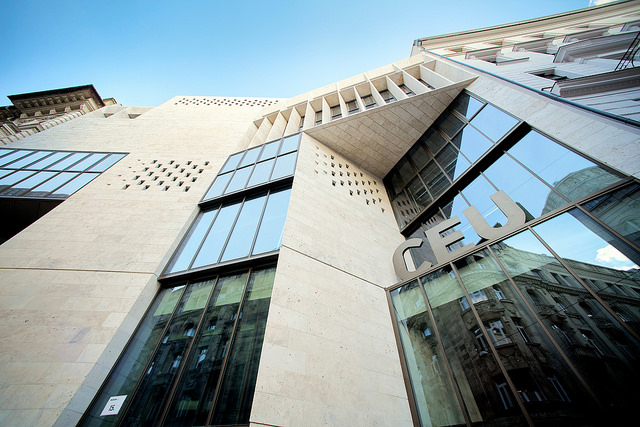
\includegraphics[scale=0.5]{figures/ceu_picture.jpg} 	% the [scale=0.5] parameter will scale the image
		\caption{A picture of CEU}
		\label{fig:ceu}
	\end{figure}


	% tables are non intuitive. Proof:
	

	\begin{center}
		\begin{tabular}{ |c|c|c| } 
		\hline
		cell1 & cell2 & cell3 \\ 
		cell4 & cell5 & cell6 \\ 
		cell7 & cell8 & cell9 \\ 
		\hline
		\end{tabular}
	\end{center}
	
	

	\end{minted}

\end{frame}


%%%%%%%%%%%%%%%%%%%%%%%%%%%%%%%%%%%%%%%%%%%%%%%%%%%%%%%%%%%%%%%%%%%%%%%%%%%%%%%%%
%%%%%%%%%%%%%%%%%%%%%%%%%%%%%%%%%%%%%%%%%%%%%%%%%%%%%%%%%%%%%%%%%%%%%%%%%%%%%%%%%

\begin{frame}
\frametitle{Adding figures and tables - output} \pause
	
\begin{figure}[h!]
	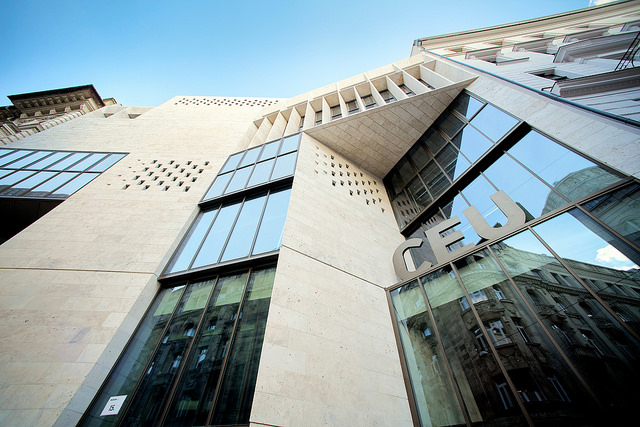
\includegraphics[scale=0.5]{figures/ceu_picture.jpg} 	% the [scale=0.5] parameter will scale the image
	\caption{A picture of CEU}
	\label{fig:ceu}
\end{figure}


\bigskip


\begin{center}
	\begin{tabular}{ |c|c|c| } 
	\hline
	cell1 & cell2 & cell3 \\ 
	cell4 & cell5 & cell6 \\ 
	cell7 & cell8 & cell9 \\ 
	\hline
	\end{tabular}
\end{center}

\end{frame}



%%%%%%%%%%%%%%%%%%%%%%%%%%%%%%%%%%%%%%%%%%%%%%%%%%%%%%%%%%%%%%%%%%%%%%%%%%%%%%%%%
%%%%%%%%%%%%%%%%%%%%%%%%%%%%%%%%%%%%%%%%%%%%%%%%%%%%%%%%%%%%%%%%%%%%%%%%%%%%%%%%%



\begin{frame}
\frametitle{Many many tools to get nicely formatted LaTeX tables} \pause
 
	\begin{itemize}
		\item \url{https://en.wikibooks.org/wiki/LaTeX/Tables#Using_spreadsheets_and_data_analysis_tools}
	\end{itemize}

\smallskip

	\begin{figure}[h!]
		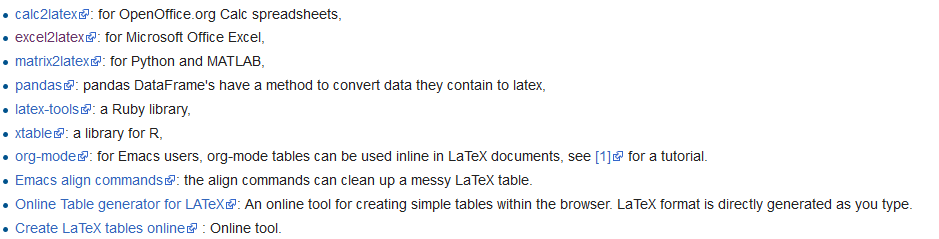
\includegraphics[scale=0.4]{tables.png}
	\end{figure}

\end{frame}


%%%%%%%%%%%%%%%%%%%%%%%%%%%%%%%%%%%%%%%%%%%%%%%%%%%%%%%%%%%%%%%%%%%%%%%%%%%%%%%%%
%%%%%%%%%%%%%%%%%%%%%%%%%%%%%%%%%%%%%%%%%%%%%%%%%%%%%%%%%%%%%%%%%%%%%%%%%%%%%%%%%


\begin{frame}
\frametitle{For everything else}
There are StackOverflow and Overleaf tutorials.
\end{frame}

%%%%%%%%%%%%%%%%%%%%%%%%%%%%%%%%%%%%%%%%%%%%%%%%%%%%%%%%%%%%%%%%%%%%%%%%%%%%%%%%%
%%%%%%%%%%%%%%%%%%%%%%%%%%%%%%%%%%%%%%%%%%%%%%%%%%%%%%%%%%%%%%%%%%%%%%%%%%%%%%%%%

\begin{frame}[t]\frametitle{Adding references with natbib}
    \begin{enumerate}
        \item Have \texttt{\usepackage[round]{natbib}} in your preambulum.
        \item You can choose the type of citation you prefer in the [param] space
        \item you add the bibliography to your document with a bibliography\{your\_bibfile\}
    \end{enumerate}
\end{frame}

%%%%%%%%%%%%%%%%%%%%%%%%%%%%%%%%%%%%%%%%%%%%%%%%%%%%%%%%%%%%%%%%%%%%%%%%%%%%%%%%%
%%%%%%%%%%%%%%%%%%%%%%%%%%%%%%%%%%%%%%%%%%%%%%%%%%%%%%%%%%%%%%%%%%%%%%%%%%%%%%%%%


\begin{frame}[t]\frametitle{How it looks like with Zotero}
	\begin{enumerate}
	\item Right click on your collection folder on the left panel
	\item 'Export collection'
	\item Format as BibTeX
	\item Save it into the same folder as your main .tex 
	\end{enumerate}
\end{frame}

%%%%%%%%%%%%%%%%%%%%%%%%%%%%%%%%%%%%%%%%%%%%%%%%%%%%%%%%%%%%%%%%%%%%%%%%%%%%%%%%%
%%%%%%%%%%%%%%%%%%%%%%%%%%%%%%%%%%%%%%%%%%%%%%%%%%%%%%%%%%%%%%%%%%%%%%%%%%%%%%%%%


\begin{frame}[t]\frametitle{How to cite with natbib}
	\begin{itemize}
		\item You can put the source in parenthesis like (Einstein 1999) with citep\{bib\_key\}
		\item Just the date, like: Einstein (1999) with citet\{bib\_key\}
	\end{itemize}
	\bigskip
	More, in-depth natbib tutorials:
	\begin{itemize}
		\item \url{http://merkel.texture.rocks/Latex/natbib.php}
		\item \url{https://www.sharelatex.com/learn/Bibliography_management_with_natbib}
	\end{itemize}
\end{frame}


%%%%%%%%%%%%%%%%%%%%%%%%%%%%%%%%%%%%%%%%%%%%%%%%%%%%%%%%%%%%%%%%%%%%%%%%%%%%%%%%%
%%%%%%%%%%%%%%%%%%%%%%%%%%%%%%%%%%%%%%%%%%%%%%%%%%%%%%%%%%%%%%%%%%%%%%%%%%%%%%%%%



\begin{frame}
\frametitle{setting up your dissertation in LaTeX}
\begin{itemize}
\item A main .tex file that contains the link to the chapters, preambulum, title page, acnowledgement, etc.
\item Each chapter is a separate .tex file
\item The .bib file with your references
\item Whatever figures and tables you want to include
\end{itemize}
\end{frame}


%%%%%%%%%%%%%%%%%%%%%%%%%%%%%%%%%%%%%%%%%%%%%%%%%%%%%%%%%%%%%%%%%%%%%%%%%%%%%%%%%
%%%%%%%%%%%%%%%%%%%%%%%%%%%%%%%%%%%%%%%%%%%%%%%%%%%%%%%%%%%%%%%%%%%%%%%%%%%%%%%%%


\begin{frame}

\centering
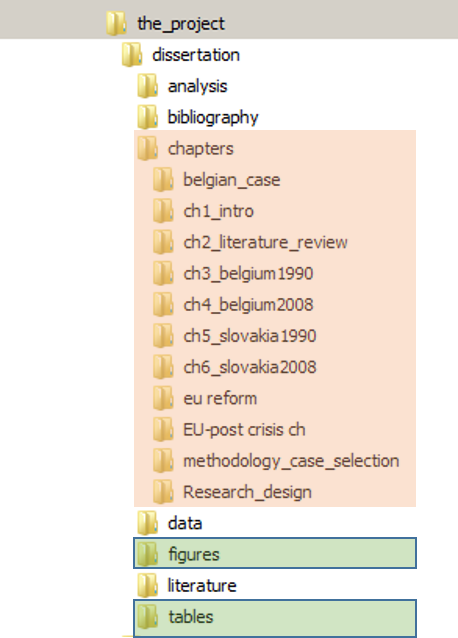
\includegraphics[scale=0.4]{figures/dissertation_files.png}

\end{frame}


%%%%%%%%%%%%%%%%%%%%%%%%%%%%%%%%%%%%%%%%%%%%%%%%%%%%%%%%%%%%%%%%%%%%%%%%%%%%%%%%%
%%%%%%%%%%%%%%%%%%%%%%%%%%%%%%%%%%%%%%%%%%%%%%%%%%%%%%%%%%%%%%%%%%%%%%%%%%%%%%%%%


\begin{frame}
Some of the advice is outdated in the CEU template if you use Overleaf or TeXstudio or other contemporary editor:
e.g.: don't worry about the order to run pdflatex and bibtex to get your final document, the software does it for you.
\end{frame}

%%%%%%%%%%%%%%%%%%%%%%%%%%%%%%%%%%%%%%%%%%%%%%%%%%%%%%%%%%%%%%%%%%%%%%%%%%%%%%%%%
%%%%%%%%%%%%%%%%%%%%%%%%%%%%%%%%%%%%%%%%%%%%%%%%%%%%%%%%%%%%%%%%%%%%%%%%%%%%%%%%%


\begin{frame}
\frametitle{The workflow with the CEU template} \pause
\begin{itemize}
	\item Have all your packages and extra formatting options in the preambulum in your main .tex \pause
	\item Decide on the citation package you want to use (I recommend either 'natbib' or 'biblatex') \pause
	\item Use your citation manager of choice (Zotero, Endnote, Mandaley, etc.) to collect your references and then export it to your .bib file \pause
	\item Finish your dissertation and graduate
\end{itemize}
\end{frame}

%%%%%%%%%%%%%%%%%%%%%%%%%%%%%%%%%%%%%%%%%%%%%%%%%%%%%%%%%%%%%%%%%%%%%%%%%%%%%%%%%
%%%%%%%%%%%%%%%%%%%%%%%%%%%%%%%%%%%%%%%%%%%%%%%%%%%%%%%%%%%%%%%%%%%%%%%%%%%%%%%%%


\begin{frame}
\frametitle{Using LaTeX for CVs, or presentations}
	You can find plenty of great LaTeX CV templates on Overleaf which you can modify after.
	\medskip
	The "beamer" class creates the presentation format (such as this one)
	\medskip
	If you want to draw great looking flowcharts or other graphics, you can use the \texttt{tikz} package
	\medskip
	All of the previous disclaimer applies to these as well: only do it if you enjoy it, or absolutely must.
\end{frame}


%%%%%%%%%%%%%%%%%%%%%%%%%%%%%%%%%%%%%%%%%%%%%%%%%%%%%%%%%%%%%%%%%%%%%%%%%%%%%%%%%
%%%%%%%%%%%%%%%%%%%%%%%%%%%%%%%%%%%%%%%%%%%%%%%%%%%%%%%%%%%%%%%%%%%%%%%%%%%%%%%%%


\end{document}

